% $Id: newproject.tex 12292 2010-09-23 12:45:32Z alexandra $
% Local Variables:
% ispell-check-comments: nil
% Local IspellDict: american
% End:
% --------------------------------------------------------
% User documentation 
% copyright by BREDEX GmbH 2004
% --------------------------------------------------------
\index{Project!New}
\index{Create!Project}
\index{Project!Create}
\index{New!Project}
\index{Project!Languages}
\index{Languages!Project}
\index{Language!Default}
\index{Default!Language}


\begin{enumerate}
\item From the \ite{}, select:\\ 
\bxmenu{Test}{New}{}.
\item If you haven't already logged into the database, a dialog will appear to ask you to do so.  \\
See the previous section \bxpref{tasksdblogin} for details. 
 
\item A wizard to create a new \gdproject{} will appear  (\bxfigref{projsettings}).

\begin{figure}[h]
\begin{center}
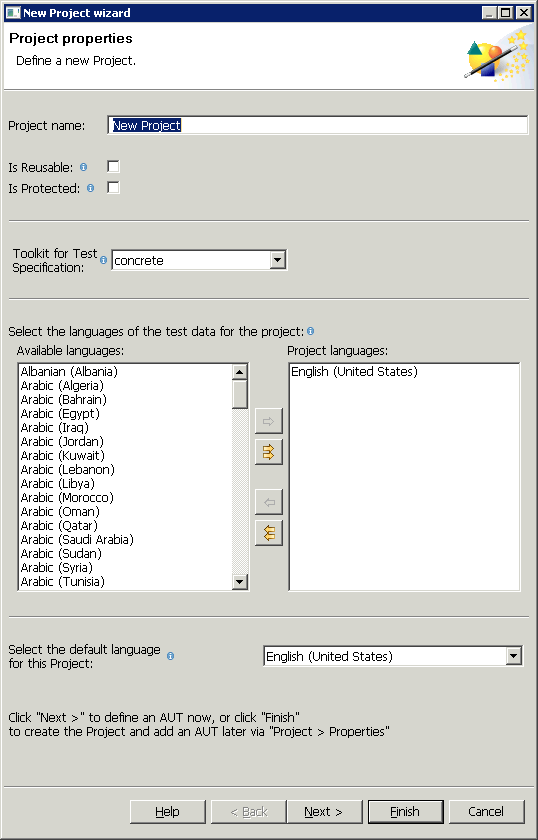
\includegraphics[width=12.5cm]{Tasks/Projects/PS/newprojectdialog}
\caption{New Project Dialog}
\label{projsettings}
\end{center}
\end{figure}

\item In the \bxname{project name} field, enter a meaningful and unique \gdproject{} name.
 Do not use any special characters in \gdproject{} names. 

\item Activate the \bxcaption{reusable project} checkbox if you want to be able to reference the \gdcases{} from this \gdproject{} in other \gdprojects{}.
This will let you use  the \gdcases{} in this \gdproject{} as the basis or library for other \gdprojects{}  (see the section later for more details on this \bxpref{reuseproject}). 

\item Choose whether this \gdproject{} should be protected. In a protected \gdprojects{}, you cannot delete \gdcases{} or edit parameters for \gdcases{}. This is only necessary if the \gdproject{} is reused in another \gdproject{} -- the protection ensures that irreversible changes cannot be made to the reused \gdproject{} that would adversely affect its dependent \gdprojects{}.

\item Select the toolkit your \gdproject{} will use from the combo box. The toolkit is the library used to create the GUI. 

\textbf{Toolkits for \gdprojects{}}\\
\label{projtoolkit}
The default toolkit is \bxname{concrete}. Choose this if you want to write \gdcases{} that can be used for different applications (e.g. for Swing and for RCP).

Choose another toolkit if you want to write \gdcases{} just for a Swing, SWT, RCP or HTML application. 

The choice of toolkit you make here will determine what actions are available to you to specify your tests. If you choose \bxname{concrete}, you will not be able to specify tests for components specific to HTML or SWT.

\item From the list of available languages, select the languages supported by your \gdaut{} and move them into the \bxcaption{project language} box using the arrow button. Use \bxkey{Ctrl} to select multiple languages.

You will be able to start the \gdaut{} in these languages, and translate test data into these languages. 


\item Select a default language from the combo box. The default language is the language your \gdproject{} is started in. 

\item You can now click \bxcaption{Next} to define an \gdaut{} for this \gdproject{} \bxpref{Defineaut}.
\end{enumerate}

If you want to define the \gdaut{} later, you can click \bxcaption{Finish} to create the \gdproject{} as it is. You can define an \gdaut{} later via the \gdproject{} properties under \bxmenu{Test}{Properties}{}. 

You can also edit the \gdproject{} details later in the \gdproject{} properties dialog \bxpref{projectproperties}.
\clearpage



